\documentclass{article}
\usepackage{tikz}
\usetikzlibrary{arrows,shapes}
 
%%%% pentagon using polar co-ordinates.  

\begin{document}
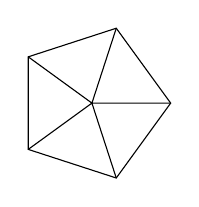
\begin{tikzpicture}
% Define the points of a regular pentagon
 
\path (0,0) coordinate (origin);
\path (0:1cm) coordinate (P0);
\path (1*72:1cm) coordinate (P1);
\path (2*72:1cm) coordinate (P2);
\path (3*72:1cm) coordinate (P3);
\path (4*72:1cm) coordinate (P4);
 
% Draw the edges of the pentagon
\draw (P0) -- (P1) -- (P2) -- (P3) -- (P4) -- cycle;
 
% Add "spokes"
\draw (origin) -- (P0) (origin) -- (P1) (origin) -- (P2) (origin) -- (P3) (origin) -- (P4);
\end{tikzpicture}
\end{document}

